%!TEX root = spack-sc15.tex

\subsection{The ARES Multi-physics Code}
\label{sec:ares}

\begin{figure*}
	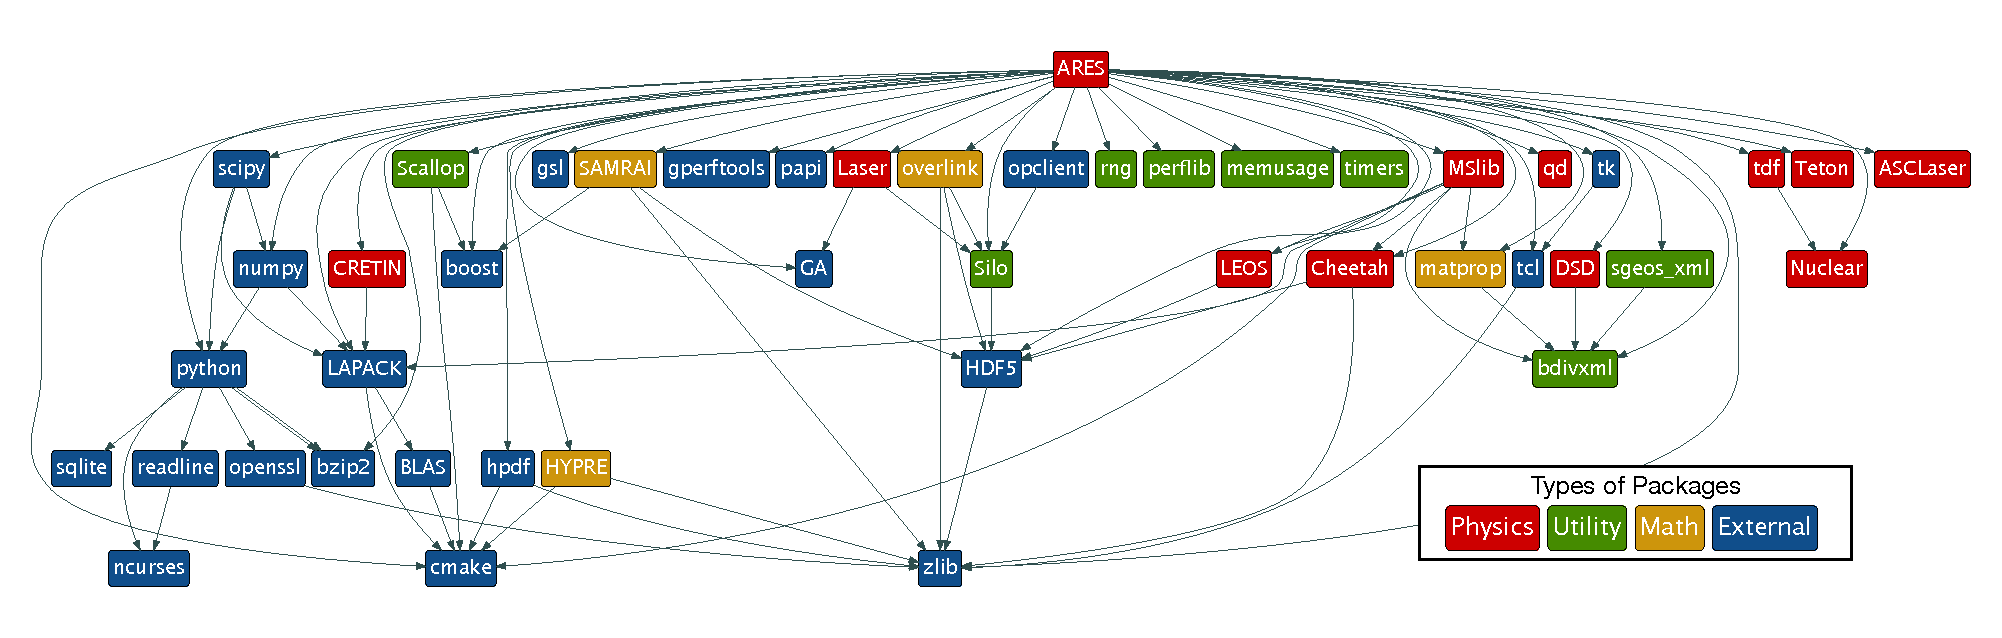
\includegraphics[width=\textwidth]{figs/ares-dot/ares-fig.pdf}
	\caption{
		Dependencies of ARES, colored by type of package.
		\label{fig:ares}
	}
\end{figure*}

\begin{table}\centering
\begin{tabular}{|r|c|c|c|c|}
\hline
\multirow{2}{*}{} & \multicolumn{2}{|c|}{\bf Linux} & {\bf BG/Q}     & {\bf Cray XE6} \\\cline{2-5}
                  & {\it MVAPICH} & {\it OpenMPI}   & {\it BG/Q MPI} & {\it Cray MPI} \\\hline
{\bf GCC}         & {\tt C P L D} &                 &                &                \\\hline
{\bf Intel}       & {\tt C P L D} & {\tt C P L D}   &                &                \\\hline
{\bf PGI}         & {\tt C P L D} &                 &                & {\tt C P L D}  \\\hline
{\bf Clang}       & {\tt C P L D} &                 & {\tt C P L D}  &                \\\hline
{\bf XL}          &               &                 & {\tt C P L D}  &                \\\hline
\end{tabular}
\caption{
	Configurations of ARES built with Spack: \newline
	(C)urrent and
	(P)revious production, (L)ite, and (D)evelopment).
	\label{tab:ares-configs}
}
\end{table}

For our final use case, we describe our experiences using Spack to build ARES.
ARES~\cite{ares1,ares2} is a 1, 2 and 3-dimensional radiation hydrodynamics code,
developed for production use at LLNL.  It is capable of running both small, serial
and large, massively parallel jobs. ARES is used primarily in munitions modeling
and inertial confinement fusion simulations.
%
At LLNL, it runs on commodity Linux clusters and on Blue Gene/Q systems.
It also runs on the Cielo Cray XE6 system at Los Alamos National Laboratory (LANL), and
it is being ported to LANL's forthcoming Trinity Cray XC30 machine on Trinitite,
a smaller version of the full system.  The Trinity machine will consist of two partitions;
one using Intel Haswell processors and another using Intel Knights Landing processors.
Currently, only the Haswell partition is deployed on Trinitite.

ARES comprises 47 packages, with complex dependency relationships.  The DAG for
the current production configuration of ARES is shown in Figure~\ref{fig:ares}.
At the top is ARES itself.  ARES depends on 11 LLNL physics packages (red),
4 LLNL math/meshing libraries (gold), and 8 LLNL utility libraries (green).
The utility libraries handle tasks including logging, I/O, and performance
measurement. In addition, ARES uses 23 external software packages, including MPI, BLAS,
Python, and many other libraries.  Together, these packages ares written in a diverse
set of languages (C, C++, Fortran, Python, tcl, etc.) using MPI and OpenMP for parallelism.

In the configuration we describe here, we have configured Spack to build ARES with
external MPI implementations, depending on the host system. This is a common
configuration, because the vendor- or site-supplied MPI installation is often
optimized and integrated tightly with network drivers on the host system. MPI is shown
as a virtual dependency in the figure, as the implementation differs according to the
host machine.  ARES builds its own Python version in order to run on machines
where Python is not well supported, like Blue Gene/Q.  In particular, ARES builds
a version of Python 2.7 for Blue Gene/Q, which is not supported by the native
software stack.

When we first began developing Spack packages for ARES and its dependencies,
the code managed its software stack using the MixDown meta-build system.
Thus, the ARES team already had some experience supporting automated builds of
dependencies. We developed Spack packages for all of the LLNL packages shown in
Figure~\ref{fig:ares}.
Many of the external packages were already available in Spack when ARES was
packaged, but some, such as Python, required modifications to support the
new platforms and compilers.

Table~\ref{tab:ares-configs} shows the configurations of ARES that we have packaged.
The rows and columns show architectures, compilers, and MPI versions.
Currently, we use the ARES Spack package to build four different configurations
of ARES: the current and previous production versions, a ``lite'' version that includes
a smaller set of features and dependencies, and a development version.  We denote these
with C, P, L, and D, respectively.  Each cell in the table indicates the
ARES configurations built for an architecture, compiler, and MPI combination.
Each different configuration of ARES requires a slightly different set of
dependencies and dependency versions, but all are supported through one common
ARES package using conditional logic on versions and variants.

Altogether, the initial packaging effort for ARES took roughly two months,
half time, for an experienced build engineer.  With 4 configurations and 8
architecture-compiler-MPI combinations, this is a total of 64 different builds.
Prior to using Spack, only the Linux/Intel configurations were automated.
In our discussions with the ARES team, they listed a number of key features
that enabled the new new platform builds to be automated:
\begin{enumerate}
\item Spack's version tracking and optional dependencies were required to
      build the four configurations with correct libraries;
\item The spec syntax allowed build scripts to concisely test compiler,
      compiler version, and dependency versions: a necessity
      for handling the particulars of different architectures;
\item Patching packages for particular platforms was
      necessary to build many packages; and
\item Using a DSL embedded in Python was a significant benefit;
      certain packages required custom scripting to patch.
\end{enumerate}

In addition to these immediate benefits, the ARES team mentioned
two potential long-term payoffs. First, using Spack allowed
the team to test with Clang.  This compiler is not currently used in
production, but we expect it to be used in production on future LLNL machines.
Testing with Clang revealed many incompatibilities, which were patched with
Spack. The team is communicating these changes back to library developers,
who will integrate them in future versions.  In this case, build automation
has allowed more testing. This helps both ARES and LLNL library developers
build more robust software.
%
Second, many of the libraries used by ARES are also used by other LLNL code
teams.  The LLNL code teams have begun creating an internal repository of
Spack build recipes to be shared.  Leveraging such a repository will
make packaging the next code significantly easier.
